\chapter{UCNA Analysis}
\label{ch:UCNA_Analysis}
%%%%%%%%%%%%%%%%%%%%%%%%%%%%%%%%%%%%%%%%%%%%%%%%%%%%%%%%%%%%%%%%%%%%%%%%%%%%%%%
%%%%%%%%%%%%%%%%%%%%%%%%%%%%%%%%%%%%%%%%%%%%%%%%%%%%%%%%%%%%%%%%%%%%%%%%%%%%%%%
%%%%%%%%%%%%%%%%%%%%%%%%%%%%%%%%%%%%%%%%%%%%%%%%%%%%%%%%%%%%%%%%%%%%%%%%%%%%%%%

\iffalse
Designing an experiment and collecting the right data are non-trivial alone,
but interpreting the results lends itself to a whole new train of thought.
The rest of this thesis is spent describing the details of such an
analysis, with this chapter summarizing important aspects,
such as terminology to be used later and the
model used to characterize our detector response.
\fi

This chapter is dedicated to introducing important aspects of the analysis that
is not strictly tied to calibrations and asymmetry extraction, but rather
data collection and processing to turn raw detector signals into values that
can be calibrated and analyzed. 





%--------------------------------------------------------------

\section{Outline of Analysis Steps} \label{sec:outline}

To preface the rest of this chapter, we can highlight
the general process of the analysis beginning with a raw detector
ADC value from each PMT and finishing with an asymmetry.
Below are the general steps:

\begin{itemize}
\item Determine pedestals for each PMT and subtract the pedestal from each data event.
\item Measure the gain of each PMT and divide the drifts out of the signal.
\item Apply a PMT-by-PMT calibration to determine the expected position dependent
  energy deposited in the scintillator
  for each event.
\item Correct for the position dependent response of each PMT
  to return a visible energy as seen by each PMT, $E_{\mathrm{vis},i}$.
\item Combine the four PMT energies into a single deposited energy, $E_{\mathrm{vis}}$.
\item Convert this combined estimate of the energy deposition to a final
  reconstructed energy, $E_{\mathrm{recon}}$, to use in analysis.
\item Calculate an asymmetry and apply all systematic corrections.
\end{itemize}

It is important to point out early on the difference between $E_{\mathrm{vis}}$ and
$E_{\mathrm{recon}}$. The deposited or visible energy, $E_{\mathrm{vis}}$, is an estimate of the energy
physically deposited in the
scintillator by a particle, while the reconstructed energy, $E_{\mathrm{recon}}$, is an estimate of
the true initial energy of an event. The two are different due to the electron losing energy
as it traverses through the windows of the decay trap, the windows of the MWPC,
the MWPC itself, and the dead layer of the scintillator. Of course the analysis could be
done in terms of $E_{\mathrm{vis}}$, but it is more convenient to express the results
in terms of the true electron energy spectrum, and also the energy dependent theory modifications
are in terms of the true initial energy of an event.




\section{Time-dependent Detector Corrections}

Obviously the system is not immune to drifts in signals due to variations
in time. There are many sources of such drifts, ranging from simple
electronic noise to changes in temperature. We deal with such time-dependent
effects using pedestal subtraction, gain correction, and constant monitoring
of backgrounds.

\subsection{Pedestal Subtraction}
The pedestal is a measure of the inherent detector signal, or baseline, 
upon which all other data signals lie. In terms of PMT signals, you can imagine 
the pedestal as a non-zero ADC value corresponding to zero input, or an offset.
You might say that the experiment can be run without caring about an offset
because the calibration will take this into account, which would be the case 
if the pedestals were constant or if we calibrated each run against itself, but 
neither is the case. We use a collection of subsequent runs to form our 
calibration sets, and these sets then calibrate data which is often taken hours,
or even days, earlier or later. Thus changing pedestals can be worrisome, and care
must be taken to determine the pedestals and subtract them from data.

To determine a pedestal, events must be chosen where there was a global trigger, but
the PMT of interest does not trigger and preferably there is no signal
whatsoever in the scintillator on that side. Obvious choices for these events are
UCN monitor triggers, opposite side two-fold PMT triggers, and high-threshold $^{207}\mathrm{Bi}$
pulser triggers from other PMTs. Once there is a global trigger, we can use the individual TDC
to ensure there was no individual trigger, and the events can be 
histogrammed for the PMT of interest. The mean of pedestal
peak can be taken as the average pedestal for a single run,
and this value can be 
subtracted from every subsequent reading of this PMT.

One interesting thing to note is that the discriminators, which determine whether
a component triggers,
for all PMTs are housed 
together, which leads to correlations between the PMT triggers. In a perfect world, 
each PMT would have one pedestal, and that pedestal wouldn't care about other PMT's signals.
Instead, what we see is that the pedestals
can be dependent on the type of events that are chosen 
to construct the pedestal, and the effect can be \~10~channels for some PMTs.
This indicates that the pedestal for one PMT may be dependent
on the signal present in another PMT. These shifts are important as a
pedestal shift of ~5-10 channels maps to an offset of roughly
~5-10 keV, as the PMTs show roughly 1:1 correspondence between ADC and keV.

The influence of event type on pedestal values means we must carefully choose which events
to use when calculating the pedestal.
The best choice would be UCN monitor events due to there being zero signal 
in the electronics box housing the PMT electronics, and these thus would give
the cleanest measurement of the PMT pedestal.
These are unfortunately the first event type we can eliminate as they are only present
during $\beta$-decay runs (when UCN are produced and thus create UCN monitor triggers)
and not during calibration runs (taken during the day when the beam is off). 
Of the remaining two options, the choice was made to use the
two-fold PMT triggers from the opposite detector rather than $^{207}\mathrm{Bi}$ pulser
events. The choice is somewhat arbitrary, because what is important is that we choose
a consistent subset of data for both calibration and $\beta$-decay data, but the
opposite side two-fold triggers do better represent the baseline present in each PMT
for data events when compared to the much higher signal present from the $^{207}\mathrm{Bi}$
pulser.


\iffalse
\begin{figure}[h] 
\centering

\includegraphics[scale=.25]{3-UCNAAnalysis/ImageHolder.pdf}
\caption{Pedestal values for a $\beta$-decay run determined using different 
types of events to illustrate the cross-talk between PMTs. (UCN Monitors, 
Bi triggers, Opposite side triggers, same side 2-fold triggers. Also shown 
is the dependence of the pedestal on which PMT triggers in the Bi Pulser. NOTE:
Choose West PMT4 in an early 2012/2013 beta run) }
\label{fig:peds_types}
\end{figure}

\begin{figure}[h] 
\centering

\includegraphics[scale=.25]{3-UCNAAnalysis/ImageHolder.pdf}
\caption{Example pedestals from all 8 PMTs}
\label{fig:peds_ind}
\end{figure}
\fi

\begin{figure}[p]
\centering
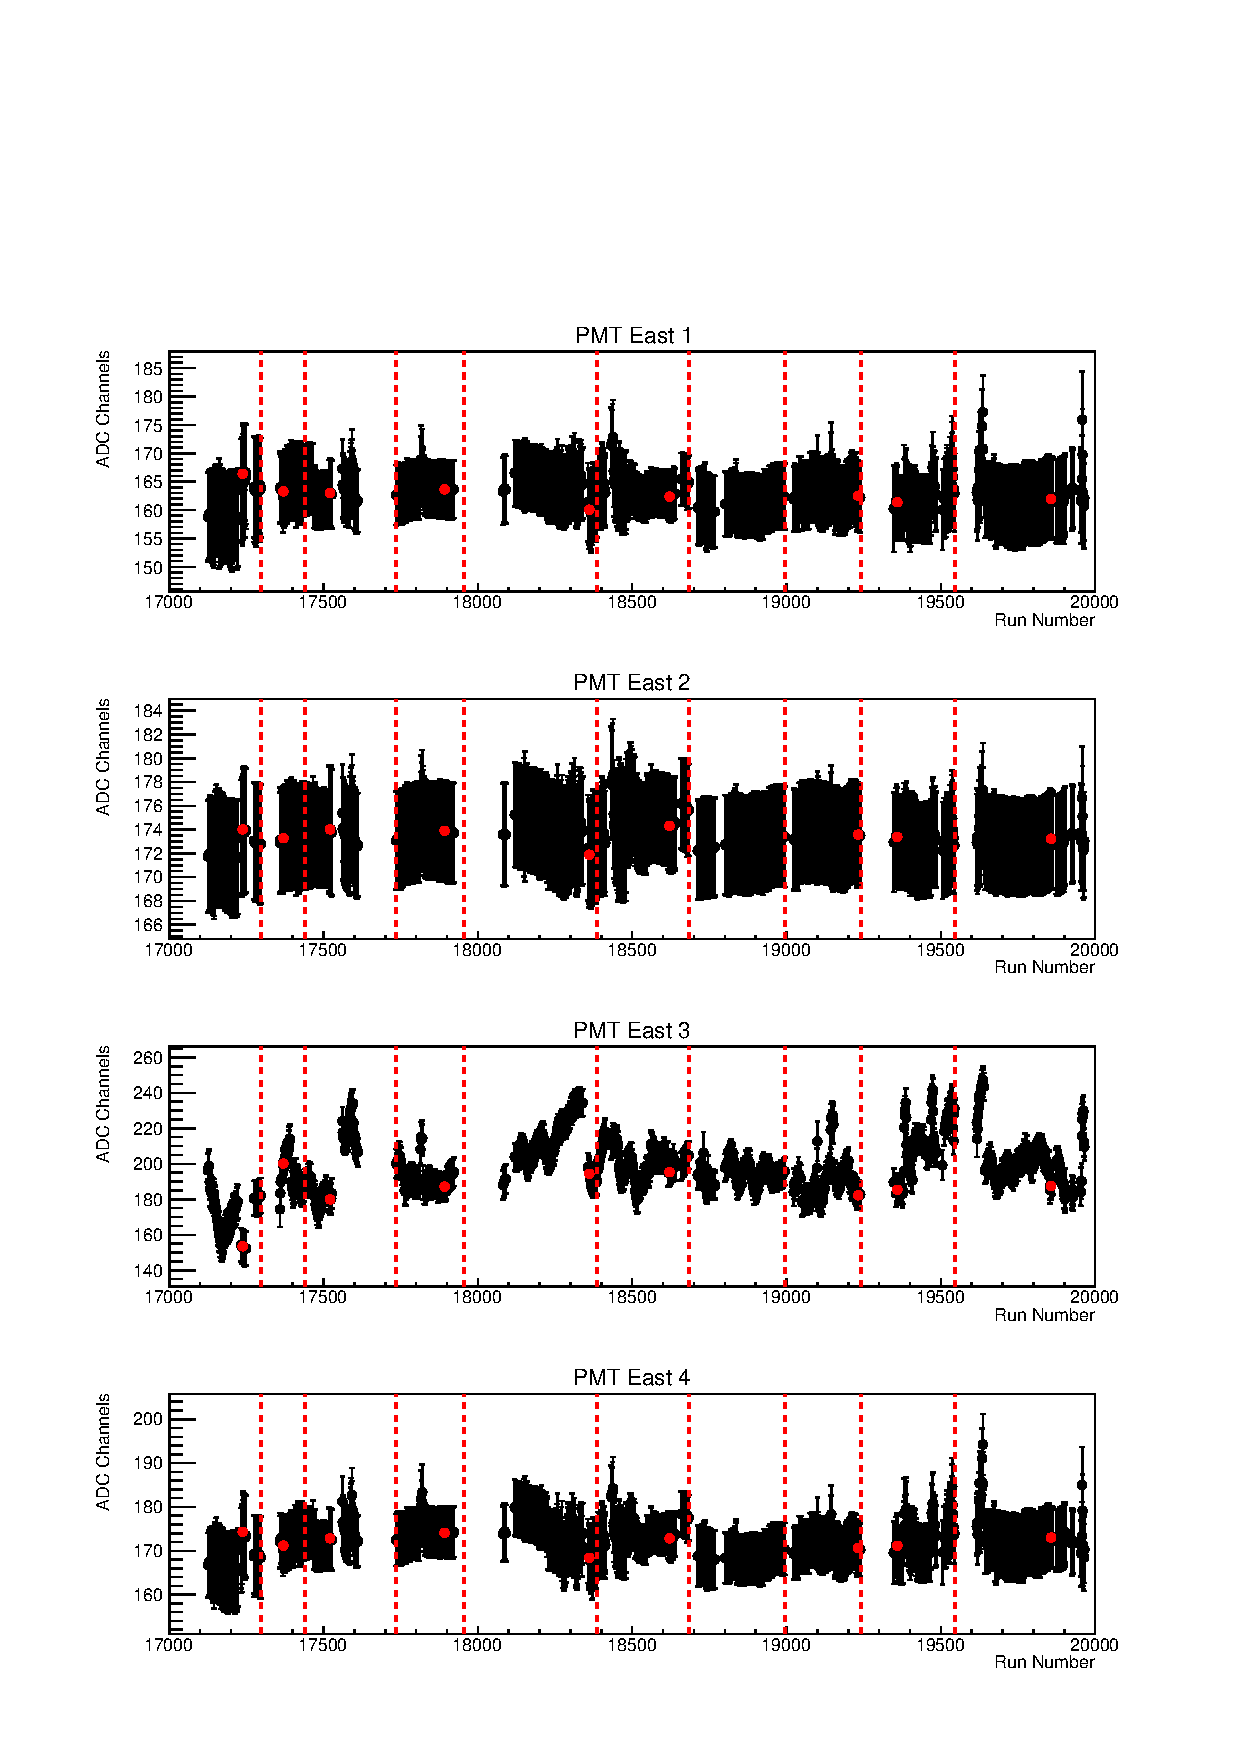
\includegraphics[page=1,scale=0.8]{3-UCNAAnalysis/2011-2012_pedestals.pdf}
\caption{Pedestal means as a function of run number for 2011-2012 East Detectors. Error bars are the
  RMS of the measured pedestal. The red lines indicate what ranges of runs belong to
  different calibration periods, and the red marker is the calibration reference run,
  which will be discussed in later sections.}
 \label{fig:peds_timeDep}
\end{figure}

\begin{figure}[p] 
\centering
\includegraphics[page=2,scale=0.8]{3-UCNAAnalysis/2011-2012_pedestals.pdf}
\caption{Pedestal means as a function of run number for 2011-2012 West Detectors. Error bars are the
  RMS of the measured pedestal. The red lines indicate what ranges of runs belong to
  different calibration periods, and the red marker is the calibration reference run,
  which will be discussed in later sections.}
\label{fig:peds_timeDep}
\end{figure}

With the event type chosen, we extract the mean and RMS of the pedestal peak
for each PMT in every run. The pedestal mean (referred to as simply
the pedestal) is then subtracted from the ADC values for all events. This effectively
removes the time-dependent baseline from the detector signals. The time dependence of
the pedestals can be seen for the East PMTs from 2011-2012 in Figure \ref{fig:peds_timeDep}.
Most of the PMTs have pedestals which remain quite stable, but PMT East 3 shows the
importance of a run-by-run pedestal subtraction.



\subsection{Gain Correction} \label{ssec:BiGain}

\subsubsection{$^{207}\mathrm{Bi}$ Pulser}
%The goal of the $^{207}\mathrm{Bi}$ gain monitoring pulser system is to create a standard
%candle type signal present in all PMTs to be tracked over time. 
The primary gain monitoring system consists of a small amount $^{207}\mathrm{Bi}$
deposited within a small block of scintillator. The scintillator was surrounded by
light reflecting material on three sides, with the fourth side covered with an optical
attenuator to attempt to match the light output of the \~1~MeV conversion line in the $^{207}\mathrm{Bi}$
to the light output of 1~MeV of energy deposited in the detector scintillator. The pulser was then
attached directly to the PMT next to where the light guides attached to the PMT.
To allow for a single-PMT high threshold trigger, the signal was split off to a different
discriminator than the one used when determining a two-fold trigger. These high threshold
discriminators then allowed for pulser triggers with a distinct pulser identification \cite{mpmThesis}.

An unfortunate but low impact issue with the pulser involves the amount of attenuation applied to the
pulser signal. The pulser peak lies well beyond the equivalent of 1~MeV of light as would be produced
in the detector scintillator, and therefore far outside the range of the $\beta$-decay spectrum. This
is not a serious issue as the PMTs seem to be quite linear, so even a peak well outside the
energy range of interest should suffice.

\begin{figure}[h] 
\centering
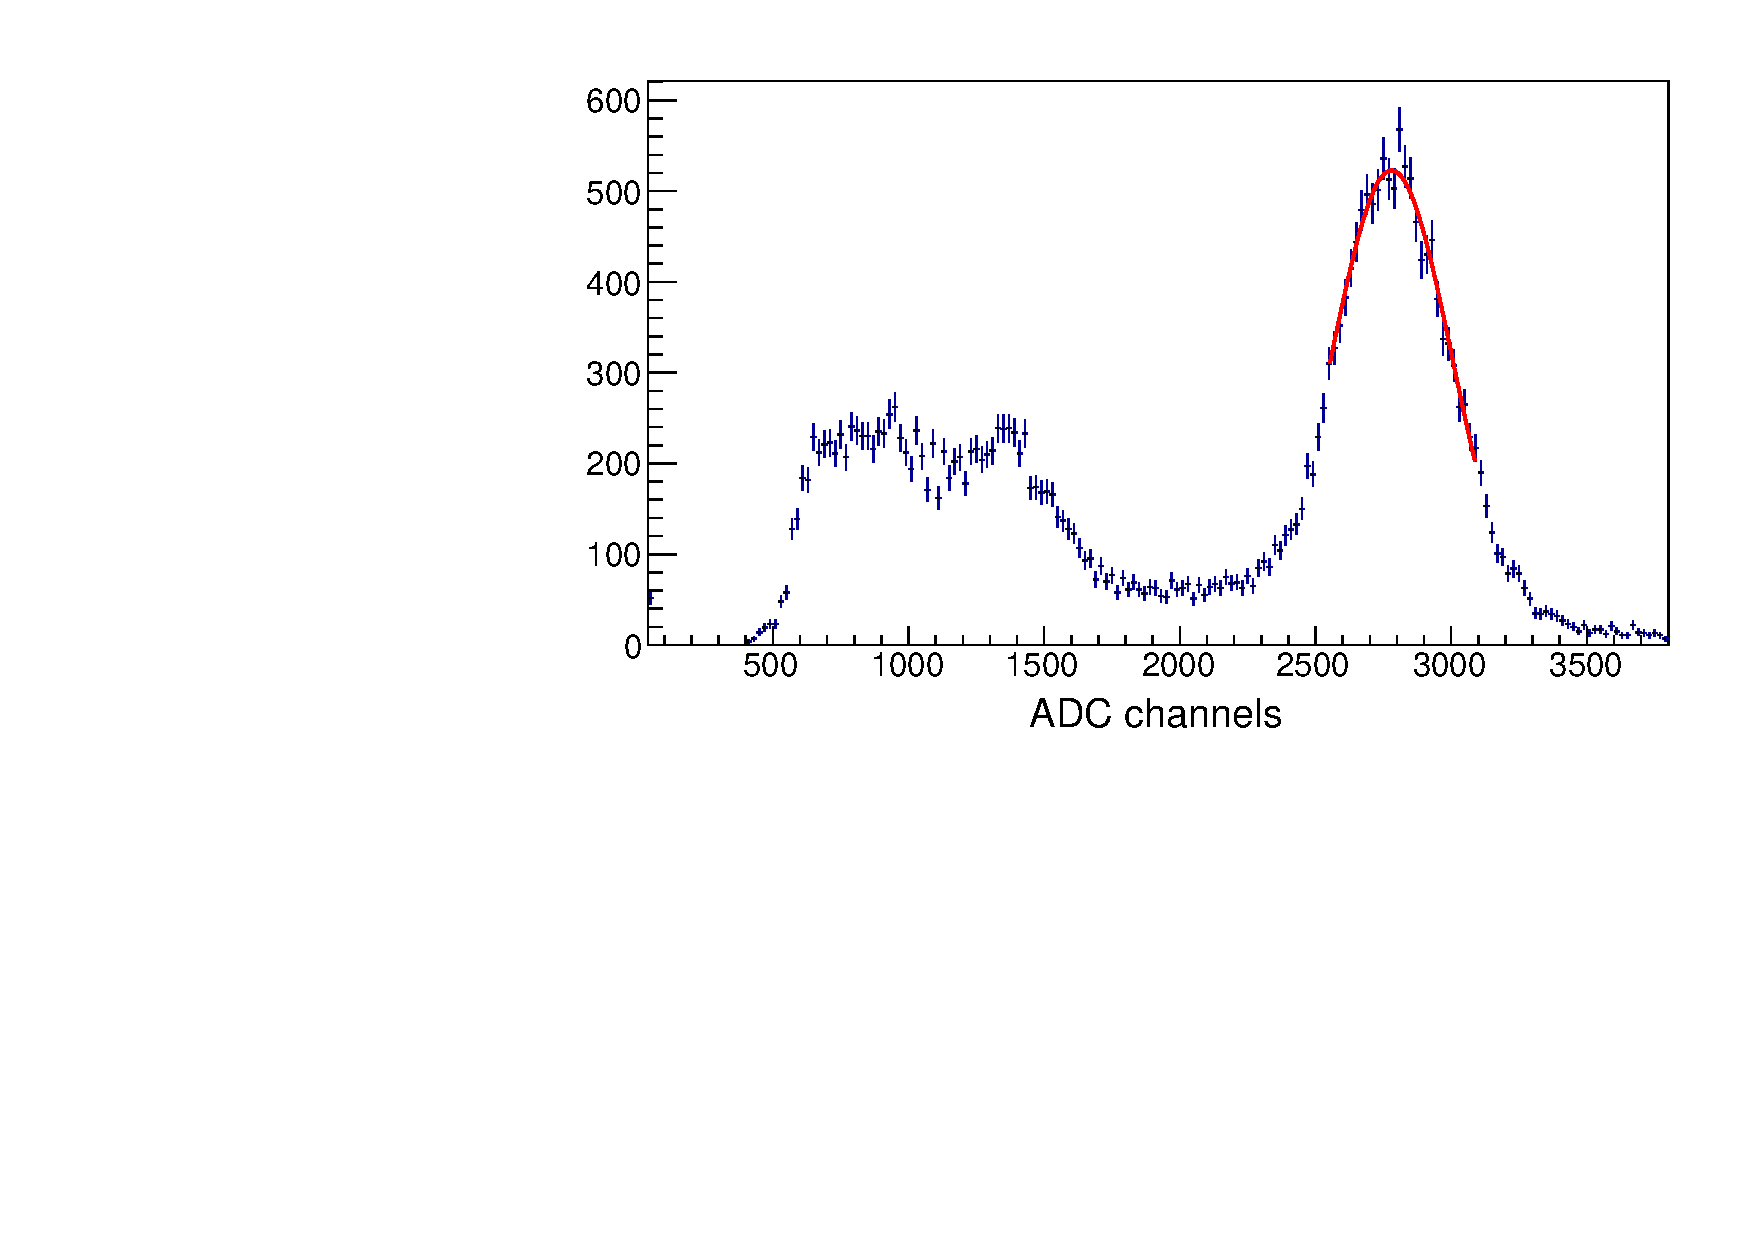
\includegraphics[scale=.60]{3-UCNAAnalysis/gain_bismuth2.pdf}
\caption{Example $^{207}\mathrm{Bi}$ spectrum and fit for a single PMT over
  the course of a run. The upper and lower bismuth conversion electron peaks are
  seen, along with a distribution from decay gammas. Note that the gamma rays are
  visible because the pulser is attached directly to PMT and there is no type
  of veto (like the MWPC) to remove them.}
\label{fig:biPulser}
\end{figure}

The $^{207}\mathrm{Bi}$ pulser peak is fit by a Gaussian on a run-by-run basis, allowing for gain corrections on the time
scale of a single run. The fit was done iteratively, with the initial guesses for mean and fit range determined
by stepping backwards from the last bin and using a self-written algorithm to search for the peak. Then the peak
was fit five times consecutively, with each successive fit being fed the previous fits mean and sigma. This
made sure the fit converged as best as possible on the mean of the pulser peak. An example pulser peak and fit
can be seen in Figure \ref{fig:biPulser}. The asymmetric fit (range extends farther above the peak than below)
is actually a characteristic part of the iterative
fitting algorithm developed for use throughout this analysis. For Gaussian like peaks occurring as a result of
a process like energy loss in a scintillator followed by PMT amplification, the upper end of the peak is
inherently more Gaussian due to the lower end having a tail from extraneous energy losses. 

The method for applying the gain correction is as follows. First, a reference gain must be determined
to normalize all other gains against. This was chosen to be what is called the ``reference run'', and it
typically consists of a manually inspected source run within each source calibration period. The gain factor
is then calculated as the ratio of the pulser peak in a given run divided by the pulser peak in the reference
run, or
%
\begin{equation}
  g_i = \frac{\mu_i}{\mu_{\mathrm{ref}}}
\end{equation}
%
This automatically defines the gain of the reference run to be $g_{\mathrm{ref}}=1$. Then all other runs which are
calibrated by a certain run period have gain factors which vary based on the fitted pulser value. The time
dependence of the gain values in 2011-2012 can be seen in figures \ref{fig:2011-2012pulser_East}
and \ref{fig:2011-2012pulser_West}. The behavior is similar in 2012-2013.

Some problems with the $^{207}\mathrm{Bi}$ pulser did occur. There were several periods where the pulser
simply did not work for a certain PMT. This was always limited to a single PMT not working, and when this
was the case the PMT without a pulser signal was not used when reconstructing the energy. This has
minimal effect on the energy reconstruction though, as the ``bad'' PMT is still used when determining
a two-fold trigger, and the remaining three PMTs contain sufficient information for reconstructing the
energy deposited. Periods where $^{207}\mathrm{Bi}$ pulser information is missing are evident in
figures \ref{fig:2011-2012pulser_West} where there is missing data for certain PMTs over extended ranges.
It should be noted that in 2012-2013, West PMT4 never had a functioning pulser.

\begin{figure}[p] 
  \centering
  \includegraphics[page=3,scale=.8]{3-UCNAAnalysis/2011-2012_gain.pdf}
  \caption{Gain factors, $g_i$, as a function of run number for 2011-2012 East Detectors.
    The red lines indicate what ranges of runs belong to
    different calibration periods, and the red marker is the calibration reference run.}
  \label{fig:2011-2012pulser_East}
\end{figure}

\begin{figure}[p] 
  \centering
  \includegraphics[page=4,scale=.8]{3-UCNAAnalysis/2011-2012_gain.pdf}
  \caption{Gain factors, $g_i$, as a function of run number for 2011-2012 West Detectors.
    The red lines indicate what ranges of runs belong to
    different calibration periods, and the red marker is the calibration reference run.}
  \label{fig:2011-2012pulser_West}
\end{figure}

\subsubsection{Endpoint Stabilization} \label{sssec:endpoint}

There are unexplained longer term gain fluctuations that do not seem to be captured by the
$^{207}\mathrm{Bi}$ gain monitoring system that can be seen by monitoring the endpoint of the
$\beta$-decay spectrum. These are corrected by applying a second gain factor, $g_{\mathrm{ep},i}$ for PMT $i$,
as the last step in the calibration process. This endpoint gain factor is determined
by comparing the endpoints as seen by each
calibrated PMT to the expected endpoint from the simulation. The final energy for each PMT
is then multiplied by this factor. This does not force the final reconstructed energy endpoint to
match the final reconstructed simulation endpoint exactly,
as the final spectra are the weighted average of the four PMT responses, but rather it corrects 
some systematically shifted periods of data which consistently exhibited endpoints $>30$~keV
away from the expected endpoint.

The method for calculating $g_{\mathrm{ep}}$ was developed previously by M. Mendenhall in section
5.2.2 of \cite{mpmThesis}. For the sake of clarity, the process is repeated here.

\begin{figure}
  \centering
  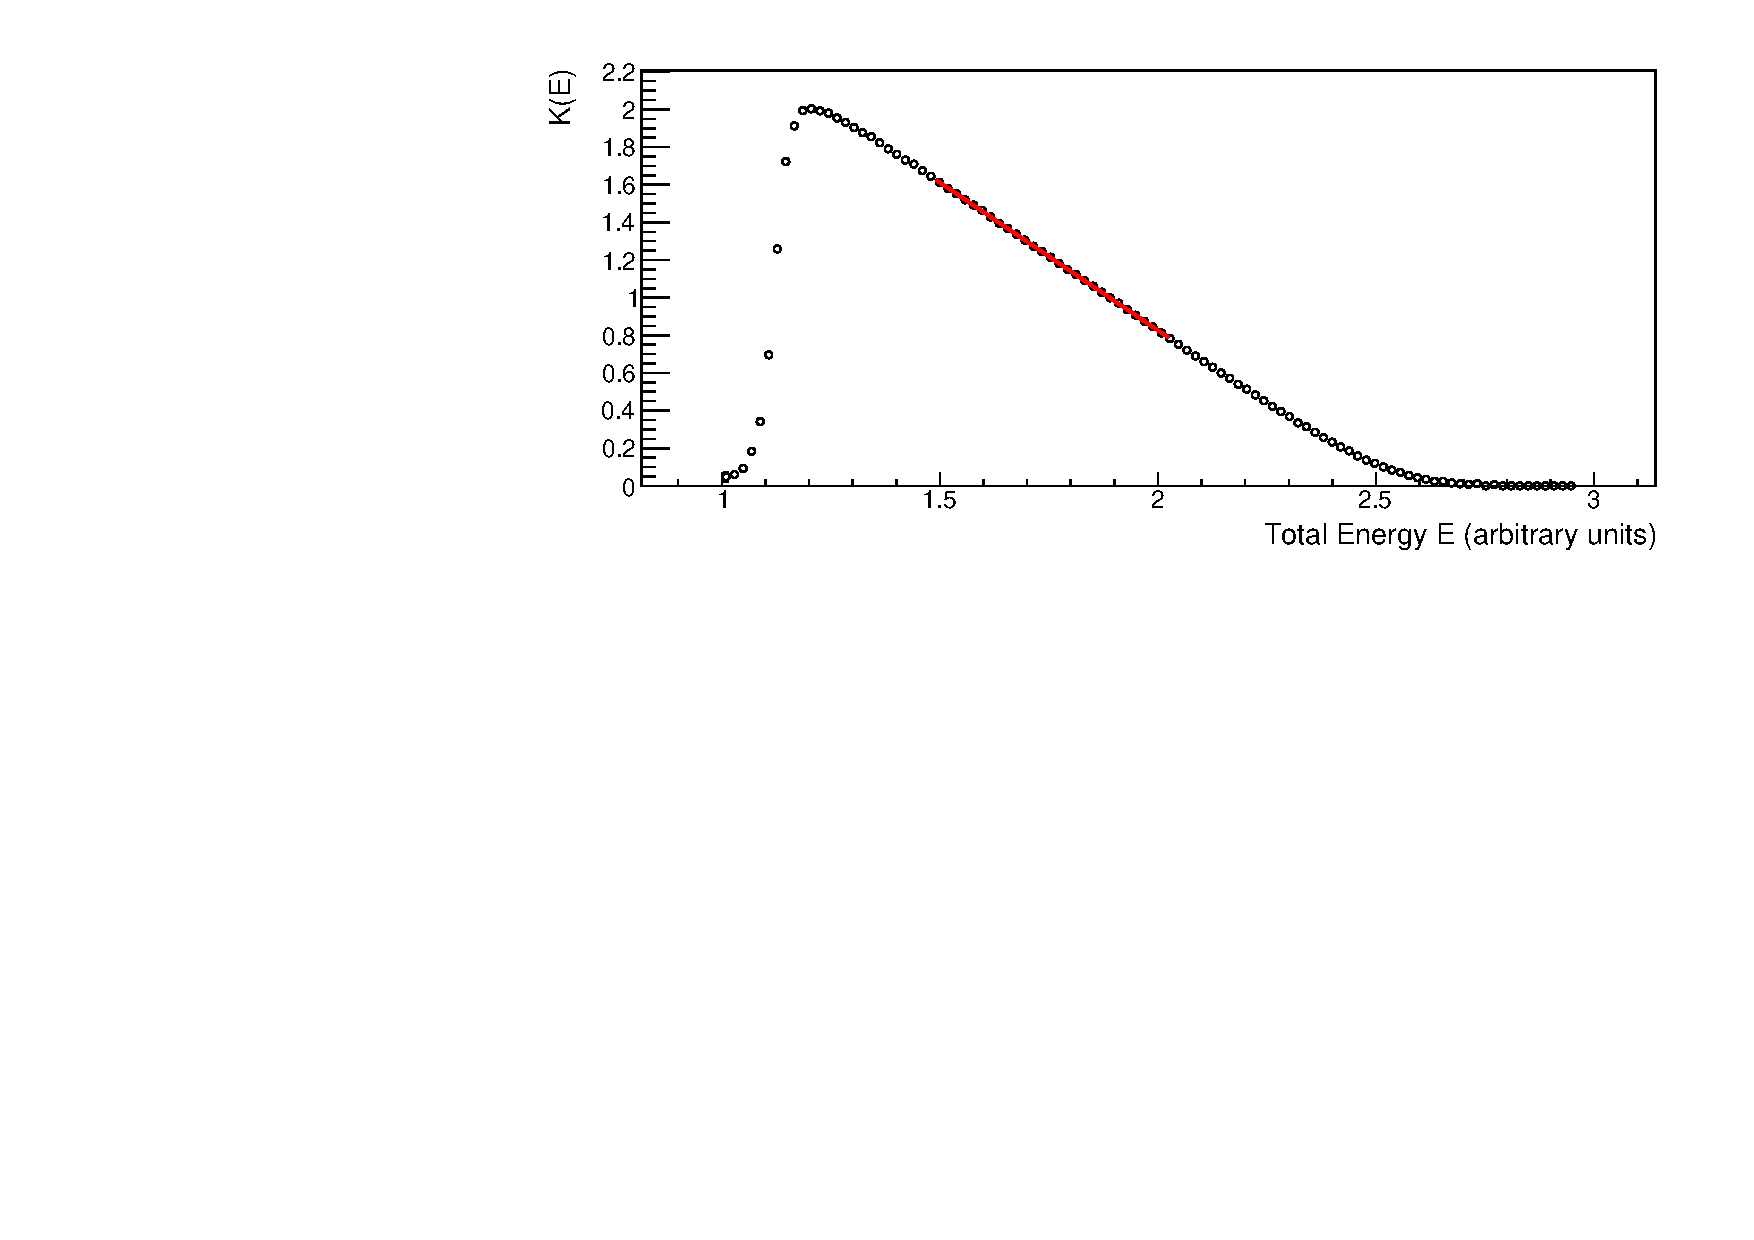
\includegraphics[scale=0.75]{3-UCNAAnalysis/kuriePlot.pdf}
  \caption{Example Kurie plot with linear fit to extract the y-intercept, which is
    the endpoint energy. The deviations from a straight line are due to the
    trigger efficiency at low energies and finite resolution at high energies. Care
    must be taken to fit in a region which more appropriately characterizes the true
    underlying electron energy spectrum.}
  \label{fig:kuriePlot}
\end{figure}
  

The endpoints are fit using a Kurie plot \cite{kurie1936radiations}, which linearizes the
energy response making for easy determination of the endpoint energy. If we approximate
the decay rate as the phase space factor for the neutron, then we can write down
the decay rate as a function of the electron total energy $E$, endpoint
energy $E_0$, and momentum $p$ as
%
\begin{equation}
  S(E) = pE\big(E_0-E\big)^2
\end{equation}
%
From this we see that a linear equation (the Kurie plot) can be formed:
%
\begin{equation}
  K(E) = \sqrt{\frac{S(E)}{pE}} = E_0-E
\end{equation}
%
where the $y$-intercept and $x$-intercept both determine the endpoint energy $E_0$.
An example Kurie plot can be seen in Figure \ref{fig:kuriePlot}.

Now we assume that the measured kinetic energy spectrum $T_{\mathrm{meas}}$ is different from the expected
kinetic energy spectrum $T_{\mathrm{sim}}$ by the gain factor $g_{\mathrm{ep}}$ such that
%
\begin{equation}
  T_{\mathrm{sim}} = g_{\mathrm{ep}} T_{\mathrm{meas}}.
\end{equation}
Then we can write the
measured total energy as
\begin{equation}
  E_{\mathrm{meas}} = m_e + g_{\mathrm{ep}}T_{\mathrm{meas}}
\end{equation}
where $c = 1$ is used. The extracted endpoint for the data is now a function of $g_{\mathrm{ep}}$
since
\begin{equation}
  K(E_{\mathrm{meas}}) = \sqrt{\frac{S(E_{\mathrm{meas}})}{pE_{\mathrm{meas}}}} = E_{0,\mathrm{meas}}-E_{\mathrm{meas}},
\end{equation}
and upon proper choice of $g_{\mathrm{ep}}$, $E_{\mathrm{meas}}=E_{\mathrm{sim}}$. To solve for
the proper gain factor, the data endpoint is iteratively fit with the gain factor adjusted upon each iteration
according to
%
\begin{equation}
  g'_{\mathrm{ep}} = \frac{ E_{0,\mathrm{meas}}- m_e}{ E_{0,\mathrm{sim}}- m_e}g_{\mathrm{ep}} =  \frac{ T_{0,\mathrm{meas}}}{ T_{0,\mathrm{sim}}}g_{\mathrm{ep}}, 
\end{equation}
%
where $E_{0,\mathrm{meas}}$ is the extracted endpoint energy from the data with gain factor $g_{\mathrm{ep}}$ applied,
$E_{0,\mathrm{sim}}$ is the expected endpoint energy extracted from simulation, $T_0$ is the endpoint kinetic energy,
and $g'_{\mathrm{ep}}$ is the guess for the next iteration of endpoint fitting.
Once the condition $1-\frac{g'_{\mathrm{ep}}}{g_{\mathrm{ep}}}<10^{-7}$ is met, the value of $g'_{\mathrm{ep}}$ is taken as the final
endpoint gain factor and is saved to the calibration database. This process is carried out for each PMT for every
$\beta$-decay run, and then every event is reprocessed with the new gain factor applied to the visible energy from PMT
$i$ according to
%
\begin{equation}
  E_{\mathrm{vis},i}^{\mathrm{FINAL}} = g_{\mathrm{ep},i} E_{\mathrm{vis},i}.
\end{equation}
Then $E_{\mathrm{recon}}$ is calcuated using the final visible energies from the available PMTs.



\subsection{Time-dependent backgrounds}
Background events which may have some time dependence are removed from the analysis
via dedicated background runs that accompany every $\beta$-decay run.
Subtracting these background rates from the data rates accounts for backgrounds
with roughly a one hour time variation.
Any backgrounds that vary at the sub one hour level may go unnoticed, but
with a signal to background better than 50:1 the contribution from such is minimal.
The background run scheme will be addressed later in this chapter, with the background
subtraction addressed in chapter 5. 

\section{Trigger Thresholds}

Looking ahead to the detector response model that will be implemented when processing
the simulated data, we need to determine the trigger thresholds for each of the
PMTs. With each PMT attached to a leading edge discriminator, the
amount of charge in a pulse that can create a trigger is randomized. The ADC signal
is an integrated signal, so two signals with integrated charge
at roughly the trigger threshold may have
different amplitudes and therefore different likelihoods of passing the discriminator threshold.
Measurement of these thresholds is important for the detector response model within the simulation
in order to properly model the low energy behavior of the measured spectrum.


\subsection{General Model for Trigger Determination} \label{ssec:genTrigModel}

The most important part of determining the trigger threshold shape for 
any detector is the availability of data which was collected no matter if 
the detector or component (PMT) produced a trigger. If such a subset of 
data is available and plentiful, it is straightforward to estimate
the trigger probability by binning the data in some unit proportional to 
energy (whether in energy or something like it isn't important) and taking 
the bin-by-bin ratio of those events that triggered to all of the events in the 
sample. Plotting these ratios as a function of whatever energy-like metric was chosen tells 
you how probable an event of some value is to create a trigger.
Once you have mapped this probability, you can then sample these curves within 
simulation to apply your true trigger threshold to simulated data.


\subsection{Trigger Data Selection}
As mentioned before, the data used for constructing trigger thresholds must not be 
biased towards triggering the PMT of interest. Thus that PMT must not be a mandatory 
component of the global trigger for that event, so care must be taken to choose only 
events which would trigger regardless of the behavior of the PMT of interest. One
other stipulation placed on these events is that they have an opportunity to 
deposit energy in a particular scintillator. The best choice of events which 
satisfy these conditions are those which have a two-fold trigger on the opposite side 
and then backscatter and those which trigger at least three PMTs on the side of 
interest, which guarantees that the scintillator would have triggered with or without 
the PMT of interest.	

\subsection{Determining the Trigger Probability}
One option for determining the trigger probability function (and probably the 
most straightforward) is to calculate the trigger probability for an entire detector as 
a whole as a function of the energy deposited by an event. What you get is a 
function that provides the probability that an event of energy $ E_i $ 
produces some sort of trigger, either 2-fold, 3-fold, or 4-fold, in that 
detector. Initially this method was used for sake of simplicity, and it produced 
reasonable agreement between simulation and data, but there is one 
glaring concern: Determining this trigger function from data requires that the data be 
calibrated first. At first glance this may not seem like much of an issue, but the 
calibration hinges upon the 
simulated peaks at low energy, which in turn rely on the trigger functions. This 
cyclical dependence hinders one from truly understanding any discrepancy between 
simulation and data at low energies, which is exactly the reason this method was 
abandoned.  

Instead, similarly to previous analyses, we decided to calculate the trigger
function on a PMT-by-PMT basis as a function of ADC channels above pedestal. This
encompasses a true characteristic of each component of the detector rather than some
average effect as seen by a detector package, which is what the aforementioned 
method produces. A typical trigger threshold is seen in Figure \ref{fig:trigger_thresh}.
As illustrated in Section \ref{ssec:genTrigModel}, the ratio of triggering events
to all events was taken in each ADC bin and then fit using the method described
in the following section.
  

\begin{figure}[h] 
\centering
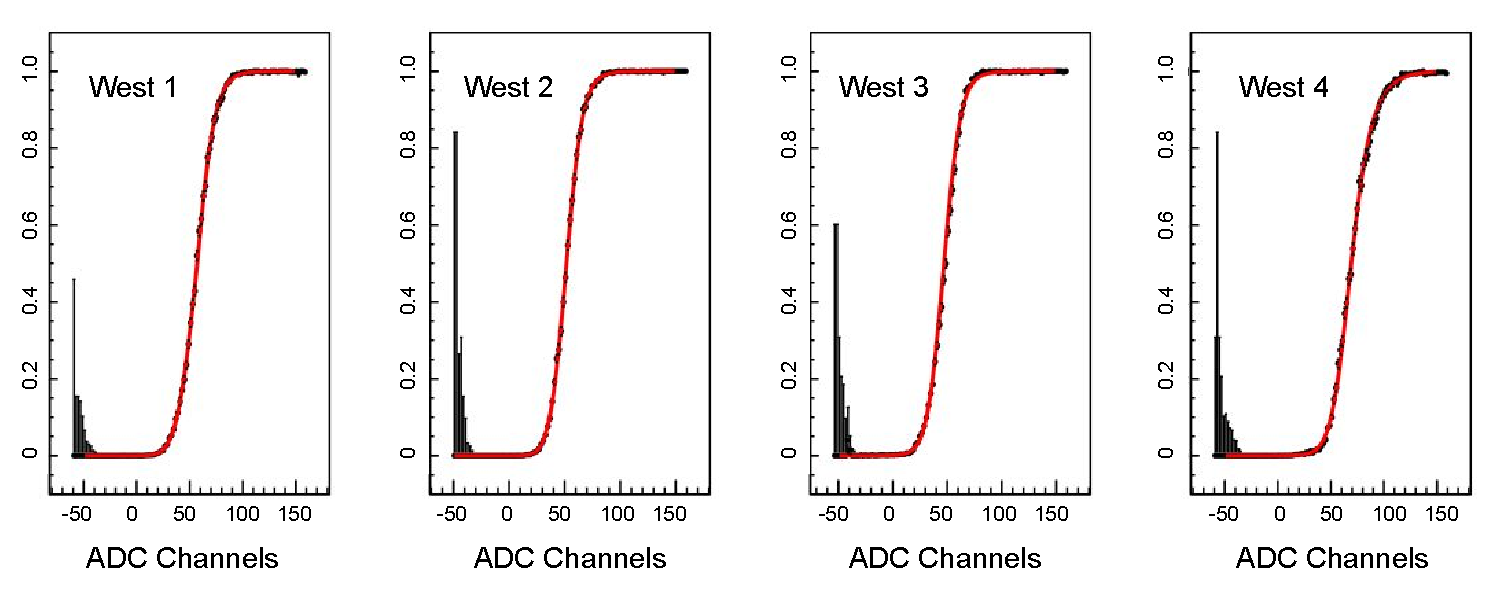
\includegraphics[scale=.6]{3-UCNAAnalysis/triggerThresholds.pdf}
\caption{Typical trigger thresholds as a function of pedestal subtracted
  ADC values from the West PMTs with fits shown in red. The y-axis
  is a probability of triggering given some ADC signal.}
\label{fig:trigger_thresh}
\end{figure}

\subsubsection{Functional Fit of the Trigger Threshold}
From the sigmoid shape of the threshold data in Figure \ref{fig:trigger_thresh}, one might guess
the shape of the curve to be a hyperbolic tangent or an error function. The data tends to show
a sharper turn on at lower ADC channels and a softer levelling off to unit probability, which
prompted the use of both the $\mathrm{erf}(x)$ (lower end of transition region)
and $\tanh(x)$ (upper end of transition region),
with a continuous transition between the
two provided by a smoothing function $S_\pm$ defined as
%
\begin{equation}
  S_\pm\big(x;x_0,R\big) \cdot f(x) = \frac{1}{2}\bigg(1\pm\tanh\Big(\frac{x-x_0}{R}\Big)\bigg) \cdot f(x),
\end{equation}
%
which acts to ``turn on/off'' ($+/-$) a function $f(x)$ around the pivot point $x_0$ and with the severity of
the on/off transition determined by the width parameter $R$. The functional fit $F(q)$ then becomes (note that the $\mathrm{erf}(x)$ and $\tanh(x)$ 
have the range (-1,1), so they must be shifted and the range halved to accomodate $0<F(q)<1$):
%
\begin{equation}
  F(q) = \frac{1}{2} \Bigg[ S_-\big(q;\mu,R\big) \bigg(1 + \mathrm{erf}\Big(\frac{q-\mu}{w_1}\Big)\bigg) +
  S_+\big(q;\mu,R\big) \bigg(1+\tanh\Big(\frac{q-\mu}{w_2}\Big)\bigg)\Bigg]
\end{equation}
%
where $q$ is the ADC value and
the free parameters are $\mu$ ($f(q=\mu)\approx 0.5$), $w_1$ (width of $\mathrm{erf}$), $w_2$ (width of $\tanh$), and $R$ (severity of turn on/off).
This function, while motivated purely by inspection of the shape of the trigger threshold, fits the data
quite well with only these four free parameters. An example of the fits for a single $\beta$-decay
run can be seen in Figure \ref{fig:trigger_thresh}. 

%-----------------------------------------------------------


\section{Simulation}
\label{sec:Simulation}

The simulations and application of the
detector response model provide a suitable starting
point for discussing the analysis, as the calibration of the data hinges
strongly on the simulation results. There is a notable dependence of the
response model on data, but this will be addressed as needed
when describing the calibration.

The simulation work for this thesis was completed
using the Geant4 simulation software package. The geometry of the
apparatus was duplicated
to the best precision possible and benchmarked against data after
the detector response model was applied. The structure
of the simulation code did not change from those in the previous analysis
as described in \cite{mpmThesis}, although minor changes were
made to the geometry to reflect real adjustments to the experimental
apparatus. 

\subsection{Input}
\subsubsection{Conversion Electron Sources}
make sure to show figures or a table with the conversion lines
\subsubsection{Activated Xenon}
\subsubsection{$\beta$-decay Electrons} \label{sssec:betaSim}

\subsection{Output}
The Geant4 simulation provides adequate trajectory tracking along with
the energy deposition along these tracks. Obviously we have access to far
more information in the simulation than we do with actual data, so the first
task is to construct observables related to those coming from the detectors.

\subsubsection{Energy Deposition}
By tallying the energy deposited along an entire track within some subset
of the geometry, one can reconstruct the energy deposited anywhere within
the SCS. The areas of highest interest for the sake of analysis are the
wirechambers and the scintillators. The energy deposited in the scintillator
is of utmost importance, as the analysis can be completed without knowledge
of the energy deposition in the wirechamber, where determination of energy
deposition is only used for type II/III separation. From here on,
the energy lost in the scintillator, as determined from simulation, will be
referred to as $E_{dep}$. This is the maximum energy which could be detectable
for an event in the data if no inconspicuous energy losses existed.

\subsubsection{Quenched Energy} \label{sssec:Equenched}
Show Birk's law. Talk about MPM and jianglai's analysis to determine
quenching parameters. Then talk about the modification using BradF's note
and show the shift to the functional form. Also show a figure which shows
the quenched energy vs Edep.

\subsubsection{Magnetic Field} \label{sssec:simMagField}

\subsubsection{Position of Detector hits}
Talk briefly of importance of position dependence, and maybe address
the way the position for the wirechamber and scintillator are calculated.
I believe this was a weighted average of the track positions where the
weights are given by the energy deposition.

\subsection{Simulating Detector Response}
While all pertinent components of the experimental apparatus were included
in the simulation, the detector response is not inherent within our
output. You may notice from (figure with quenched energy) that this
doesn't resemble the gaussian peaks normally seen in a detector signal.
The gaussian-like peaks arise from finite resolution effects and
must be put in defacto using parameters calculated
from real data. The better we understand the conversion from a pure simulation
energy output to a response which mimics that from our actual detectors, the
more credence we can put in our calibration. For the time being, the model will
be introduced with parameter determination addressed as it arises. 

\subsection{Detector Response Model}

Recall from Section \ref{sssec:pmtModel} that we can relate a digital signal
in a PMT, $ADC_i$, to the energy deposited in the scintillator
using Equation \ref{eq:EnergyResponse}.
By reverse engineering this process, we can use a purely simulated $E_Q$ and
simulate an ADC channel, so that we can process the simulated data in
exactly the same way we process real data. The following equation comes directly
from \ref{eq:EnergyResponse}:

\begin{equation} \label{eq:pmtResponse}
ADC_i = f_i^{-1}\left(\eta_i(x,y) \cdot E_{Q} \right)/g_i(t) + p_i(t) + \delta p_i(t) 
\end{equation}

This relationship is somewhat incomplete though, as it does not address the
stochastic nature of the PMTs themselves. Let's rewrite ************To properly incorporate this into our
model we must utilize the fact that a PMT consists of several dynodes, each of which
introduces stochasticity into the final voltage read out. 



%----------------------------------------------------------

\section{Energy Response from Detector Response} \label{sec:EnergyResponse}
Following the process outlined in the previous section, we can derive an
expression which takes a detector signal to an energy estimate for each PMT.
The visible energy $E_{\mathrm{vis},i}$ deposited
in the scintillator as seen by a single PMT $i$ for an event at position $(x,y)$ 
is given by the following: 

\begin{equation} \label{eq:EvisResponse}
E_{\mathrm{vis},i} = \eta_i^{-1}(x,y) \cdot f_i\bigg( \Big( \mathrm{ADC}_i - p_i(t) \Big) \cdot g_i(t) \bigg)  ,
\end{equation}

\noindent where 
\begin{align*}
  &f_i = \text{linearity relation from ADC channels to light output (proportional to energy),}\\
  &\eta_i(x,y) = \text{PMT position map factor to correct for position dependence of light response,} \\
  &p(t) = \text{mean pedestal value for PMT } i,\\
  &g(t) = \text{gain correction factor for PMT }i.
\end{align*}

This expression is exact in the case where all values are determined with infinite
precision and without stochastic fluctuations. Unfortunately, each parameter on the right
side of this equation is either stochastic in itself (as is the ADC response), or it was
determined via observation of a random process (the gain and pedestal), and so
the underlying value for any given event may not be the same as the value applied in the
above expression. Thus what we
really resolve is an approximation to the energy, which comes with some uncertainty. This
uncertainty will be addressed later in Section \ref{ssec:energyRecon}.
For the time being, keep in mind the above list of
input parameters which take us from an ADC signal (detector signal) to an energy signal. 

\subsection{Combining PMT Responses} \label{ssec:combinePMT}

For every two-fold trigger, all four PMTs from each side (eight in total) are read out by the
DAQ. Upon application of the individual detector calibrations, this yields
eight visible energies, $E_{\mathrm{vis},i}^\mathrm{E,W}$, where $i$ runs from 1 to 4 for the
four PMTs on each side. For each detector, the four available energies should
be combined to create a visible energy for each side, $E_{\mathrm{vis}}^\mathrm{E,W}$. While the
majority of events only strike one scintillator so only one of E/W visible energies will
be useful, the Type 1 events will have a usable energy on each side.

Now not all PMTs are created equal. Some PMTs have better resolution than others, thus these PMTs
should contribute more to the average energy. A simple average would not account for this, but
a weighted average, upon definition of the weights, will suffice:
%
\begin{equation}
  E_{\mathrm{vis}}^\mathrm{E,W} = \frac{\sum_{i=1}^{4} w_i E_{\mathrm{vis},i}^{\mathrm{E,W}}}{\sum_{i=1}^{4} w_i},
\end{equation}
%
where $w_i=\frac{1}{\sigma_i^2}$ are the weights for each $E_{\mathrm{vis},i}^{\mathrm{E,W}}$. We will drop the superscript
E/W for now, understanding that what follows is done for each detector.

Now let's assume that the $E_{\mathrm{vis},i}$ from Equation \ref{eq:EvisResponse} is an approximation
for an event which deposited exactly the energy $E_Q$ (the $Q$ stands for ``quenched'', which will
be described in Section \ref{sssec:Equenched}). A certain amount of this $E_Q$ is visible to each
PMT, given by $\eta_i(x,y)E_Q$, as each PMT only captures a portion of the total number of photons produced
in the scintillator.
Now if we want to relate this to the signal read out by the DAQ
from the PMT, we must multiply by a PMT resolution factor $\alpha_i$ to convert from energy
to photoelectrons, giving $N_i = \alpha_i \eta_i(x,y) E_Q$.
These PMT resolution factors are calculated during the calibration process
and will be discussed in Section \ref{ssec:PMTresolution}, but for now, assume they are known.

The number of photoelectrons produced by a PMT is a stochastic process, so we can write the actual
measured number of photoelectrons as $\overline{N_i} = N_i \pm \sqrt{N_i}$. The fractional uncertainty
is then $1/\sqrt{N_i} = 1/\sqrt{\alpha_i \eta_i(x,y) E_Q}$. Now, since the measured number of photoelectrons,
$\overline{N_i}$, is directly proportional to the ADC signal of the PMT and thus also the visible energy
of the PMT by Equation \ref{eq:EvisResponse}, we have
%
\begin{equation}
  E_{\mathrm{vis},i} = E_Q \pm \frac{E_Q}{\sqrt{\alpha_i \eta_i(x,y) E_Q}} =  E_Q \pm \sqrt{\frac{E_Q}{\alpha_i \eta_i(x,y)}}.
\end{equation}
%

The measured value of $E_{\mathrm{vis},i}$ is actually sampled from a distrubution with $\mu$ and $\sigma$ given by the
above equation, but we can assume that the best weight is given by $w_i = \frac{1}{\sigma_i^2} = \frac{\alpha_i \eta_i(x,y)}{E_Q}$.
Then the final combined $E_{\mathrm{vis}}$ for a single detector becomes
%
\begin{align}
  E_{\mathrm{vis}} &= \frac{\sum_{i=1}^{4} \frac{\alpha_i \eta_i(x,y)}{E_Q} E_{\mathrm{vis},i}}{\sum_{i=1}^{4} \frac{\alpha_i \eta_i(x,y)}{E_Q}}
  = \frac{\sum_{i=1}^{4} \alpha_i \eta_i(x,y) E_{\mathrm{vis},i}}{\sum_{i=1}^{4} \alpha_i \eta_i(x,y)} 
  = \frac{\sum_{i=1}^{4} \alpha_i f_i(q)}{\sum_{i=1}^{4} \alpha_i \eta_i(x,y)}
\end{align}
%
where we have used Equation \ref{eq:EvisResponse} with $q=\big( \mathrm{ADC}_i - p_i(t) \big) \cdot g_i(t)$.
The uncertainty on the final weighted average above is given by
\begin{equation}
  \delta E_{\mathrm{vis}} = \frac{1}{\sqrt{\sum_{i=1}^{4} w_i}} = \frac{1}{\sqrt{\sum_{i=1}^{4} \frac{\alpha_i \eta_i(x,y)}{E_Q}}}
    \approx  \sqrt{\frac{E_{\mathrm{vis}}}{\sum_{i=1}^{4}\alpha_i \eta_i(x,y)}}.
\end{equation}

As pointed out in \cite{mpmThesis}, the position map values only enter into the weighted average
as part of the sum in the denominator and multiplied by the $\alpha_i$ conversion factors, which is a smoother
function of position than the individual position map values, and thus sensitivity to uncertainty in position map
values $\eta_i$ should be minimized.

\subsection{$E_{\mathrm{vis}}$ to $E_{\mathrm{recon}}$}

As mentioned in Section \ref{sec:outline}, $E_{\mathrm{vis}}$ is an estimate of the
energy visible to the PMT from deposition in the scintillator. The more meaningful
initial energy of the particle must be determined using a separate parameterization.
To determine such a parameterization, simulated data is used so that the initial
energies of the events are known precisely, and then the response of the detector
to different event energies and types can be modeled.

\begin{figure}[h]
  \centering
  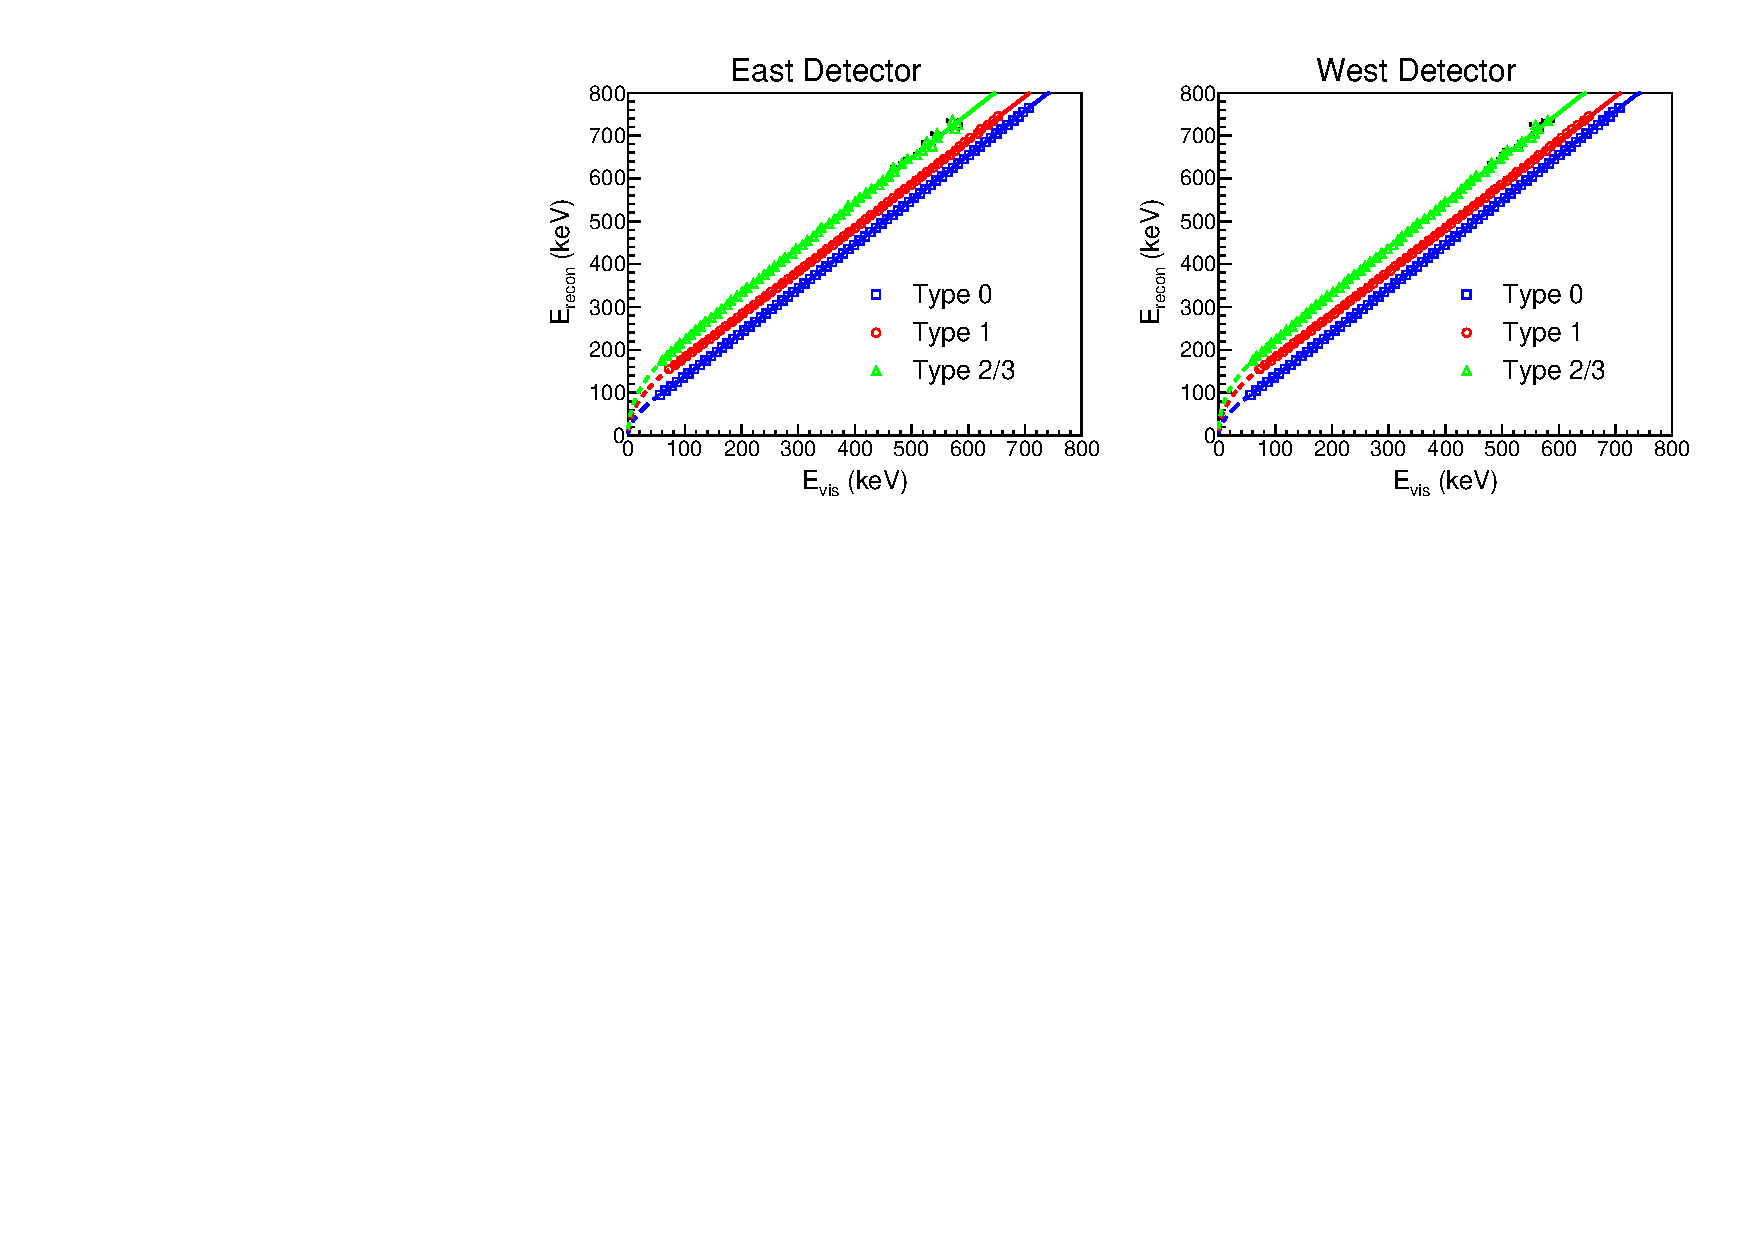
\includegraphics[scale=0.78]{3-UCNAAnalysis/2011-2012_Evis_to_Erecon.pdf}
  \caption{Parameterization between $E_{\mathrm{vis}}$ and $E_{\mathrm{recon}}$ for
    2011-2012. The mapping for the other geometries are very similar and thus are
    not shown.}
  \label{fig:Erecon}
\end{figure}

The mapping between $E_{\mathrm{vis}}$ and $E_{\mathrm{recon}}$ is determined separately
for 2011-2012, 2012-2013, and 2012-2013 with isobutane in the wirechamber.
Using the simulated $\beta$-decay spectrum and a characteristic set of detector
response variables, the simulated events are processed in the same manner as
they would be for data. They are identified as Type 0,1, or 2/3, and their
$E_{\mathrm{vis}}$ values for each detector are determined. Then the events are
grouped into histograms using their initial energy (we will call it $E_{\mathrm{recon}}$,
but really this is the true energy of the events), with the histograms corresponding
to 10~keV groups from 0~keV to 790~keV. Then each of these histograms are fit to
determine the average $E_{\mathrm{vis}}$ value for a given $E_{\mathrm{recon}}$. The results
of these fits for each event type in each detector for 2011-2012 is shown as the data
points in Figure \ref{fig:Erecon}. The other geometries look very similar and thus are
left out. Data points with low statistics at low energies were dropped.

The fit to the data is of the form
\begin{equation}
  E_{\mathrm{recon}} = C_1 + C_2E_{\mathrm{vis}} + \frac{C_3}{E_{\mathrm{vis}}} + \frac{C_4}{{E_{\mathrm{vis}}}^2},
\end{equation}
and then the fit is extrapolated continuously to zero from the lowest energy data point using
\begin{equation}
  E_{\mathrm{recon}} = C_5{E_{\mathrm{vis}}}^{C_6}
\end{equation}
with the parameters $C_5$ and $C_6$ determined by ensuring the two equations are equal at the
transition point along with their first derivatives.

Using the fitted parameters, an $E_{\mathrm{recon}}$ value is determined
for every event by plugging its weighted average $E_{\mathrm{vis}}$ into the proper equation.
It should be noted that for Type 1 events, the visible energies of both the East and West
detectors are added together when determining the parameterization, so
the same is done when applying the above parameterization to data. This is done to utilize as much
detector information as possible. The side for a Type 1 event is set to
the detector with the earlier trigger, making it the primary detector.
Thus, for a Type 1
event, one would plug $E_{\mathrm{vis}} = E_{\mathrm{vis}}^E + E_{\mathrm{vis}}^W$ into the $E_{\mathrm{recon}}$
equation for the side that triggered first.


%---------------------------------------------------------------------------------------


\section{Calibration Overview}

In the next chapter, we will take an in depth look at the calibrations of both
the wirechamber and the scintillator. Here we simply highlight their use in the analysis.

\subsection{PMT Calibration} \label{ssec:PMTCal}

The PMT calibration, as mentioned in Section \ref{sssec:scintEnCal},
uses well known conversion electron sources
to understand the detector response to there well-defined energies. By comparing the detector
response (coupling both ADC values and position map values) to simulated responses,
we can map ADC signals from each PMT to visible energies deposited
in the scintillator. These calibrations parameterize the detector response so that the
functional form of the calibration can be applied to the $\beta$-decay data.

\subsection{Wirechamber Calibration}

The wirechamber calibration relates the anode signal in the MWPC to an energy deposited in the MWPC. This is
primarily useful for separating the Type 2/3 backscattering events, as the
energy deposition in the MWPC is not used within the reconstruction of an electron's initial
energy. This separation is important though as it drastically reduces the systematic
correction for these backscattering events.
 

\section{Polarimetry} \label{sec:polarimetry}

The polarimatry analysis was carried out Eric Dees of North Carolina State University and
deserves the attention of an entire dissertation itself. The previous polarimetry measurement
is described in detail in a dissertation by Adam Holley \cite{holley2012ultracold}. A major
difference between the previous depolarization measurement and the current depolarization
hinges upon the installation of the shutter between the spin flipper and decay trap. An
update of the new polarimetry measurement method can be found in the publication of the result
presented within this dissertation \cite{brown2017}.

\begin{figure}[h] 
\centering
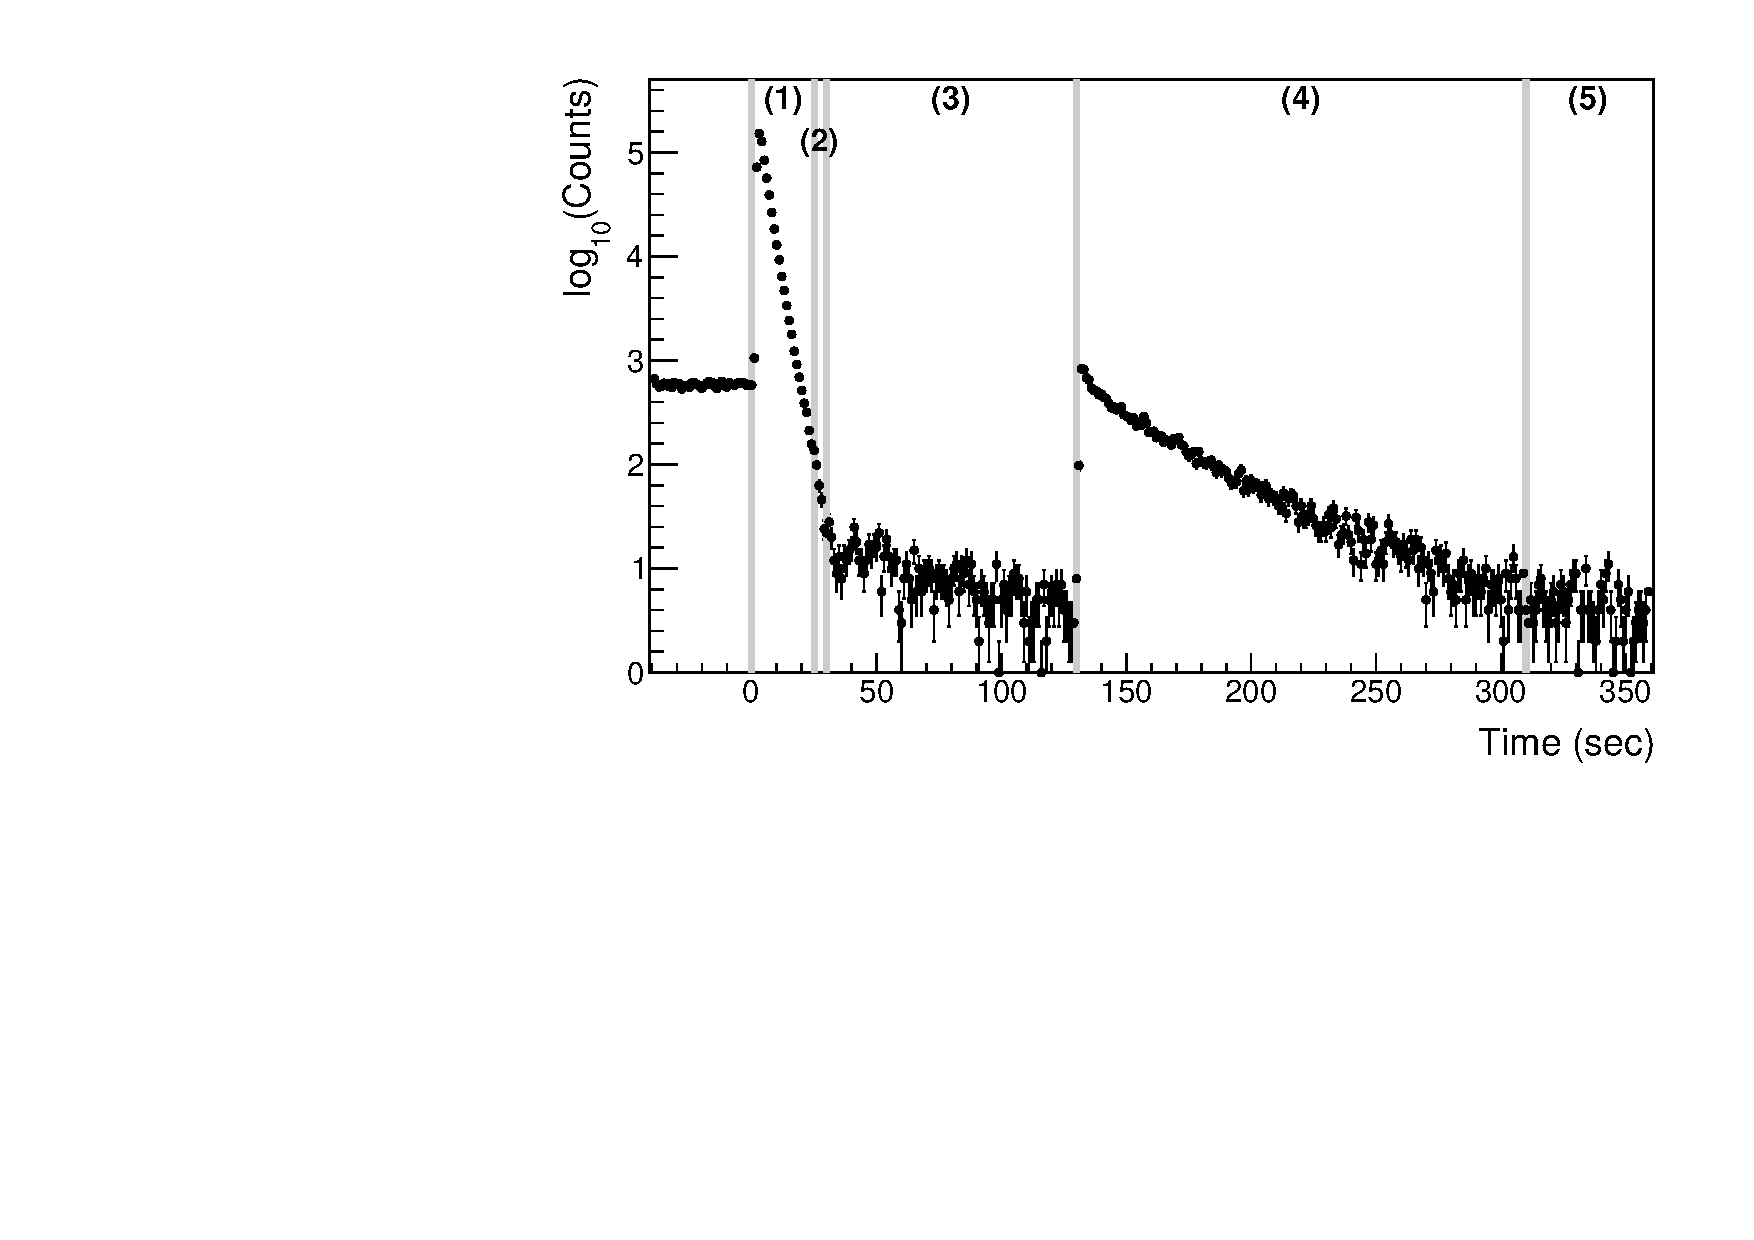
\includegraphics[scale=.55]{3-UCNAAnalysis/Switcher_signals.pdf}
\caption{Figure courtesy of E. Dees and A. R. Young as published in \cite{brown2017}.
  ``Switcher signal as a function of time, during ``D''-type runs: (1) the shutter
  closes and the switcher state changes, permitting UCN in the
  guide outside the decay volume to drain to the switcher UCN detector, (2) the AFP
  spin-flipper changes state, allowing depolarized neutrons in the guides outside the
  decay volume to drain to the switcher, (3) the shutter opens, permitting depolarized
  neutrons within the decay volume to drain to the switcher detector, (4) the AFP
  spin-flipper returns to its initial state, allowing the initially loaded spin state
  to drain from the decay volume, (5) backgrounds are measured after the UCN
  population in the decay volume has drained away.  The presented data were taken in 2011
  and UCN loaded into the decay volume with the spin-flipper off.''}
\label{fig:switcherSignal}
\end{figure}

Here is a brief description of the polarimetry measurement.
The polarimetry measurement determines the average neutron polarization in each spin state using
the depolarization runs that follow every $\beta$-decay run. As detailed in section
\ref{sec:polarization}, the neutrons are initially polarized by traversing the 7~T primary
polarizing magnet, and then the desired spin is chosen using the AFP spin flipper.

After a $\beta$-decay run, the depolarization run begins by closing the shutter and changing the switcher
state to allow
the UCN to flow into the switcher detector for measurement of UCN populations. The switcher signal
as a function of time can be found in Figure \ref{fig:switcherSignal}. The guides are cleaned of UCN while
the UCN population in the trap remains contained. Then the spin flipper state is changed allowing the
neutrons that were trapped between the 7~T magnet and the decay trap to pass back through the high
field region (these trapped neutrons result from UCN who underwent an unwanted spin flip after passing
the high field region, subsequently keeping them passing the 7~T field). Now that the guides are cleaned,
the shutter is opened and all UCN with spins not equal to the desired loaded spin are emptied (remember that
the spin flipper is switched from its original state). Once this population has been measured in the
switcher detector, the spin-flipper state is again changed back to its original state, and the
properly polarized UCN population is measured in the switcher detector. This process is followed by a short
background measurement in the switcher detector.

The ratio of these populations is then extrapolated back to the equilibrium population as established
during $\beta$-decay running by utilizing further \textit{ex situ} measurements and comparisons with
simulation. The results of these measurements as well as the correction to the uncertainty resulting
from imperfect polarization ($P<1$) can be found in Section \ref{ssec:polCorr}.





